\subsection{Información general del MCU}
En la siguiente práctica de laboratorio se utiliza el microcontrolador de ATmel AT-tiny4313 como elemento central de la práctica. Posee las siguientes caracterísiticas:
\begin{itemize}
    \item Microcontrolador AVR de 8 bits con microarquitectura RISC/Harvard \cite{presentacion}.
    \item Memoria: 2/4Kb de Flash, 128/258 bytes de SRAM y 128/258 bytes de EEPROM \cite{presentacion}.
    \item 18 GPIOs agrupados en tres puertos así como timers/counters de 8 y 16 bits \cite{presentacion}.
    \item 4 canales PWM y comparador analógico \cite{presentacion}  (No utilizado en esta práctica).
    \item USI, USART \cite{presentacion}  (No utilizado en esta práctica).
    
\end{itemize}

En figura \label{pines} se encuentra el diagrama de pines y en figura \ref{bloques} el diagrama de bloques. 


% Please add the following required packages to your document preamble:
% \usepackage{multirow}
\begin{table}[H]
\centering
\begin{tabular}{|l|c|}
\hline
Voltaje de operación (V)             & 1.8 - 5.5                                       \\ \hline
Temperatura de operación                & -55C a +125C                                    \\ \hline
$V_{IL}$                                 & -0.5 a 0.2$V_{CC}$                              \\ \hline
$V_{IH}$                                 & 0.7$V_{CC}$ a $V_{CC}$+0.5                                  \\ \hline
Corriente DC por Vcc y GND Pins      & 200.0 mA                                        \\ \hline
\multirow{3}{*}{Grados de velocidad} & 0 – 4 MHz @ 1.8 – 5.5V                          \\ \cline{2-2} 
                                     & 0 – 10 MHz @ 2.7 – 5.5V                         \\ \cline{2-2} 
                                     & 0 – 20 MHz @ 4.5 – 5.5V                         \\ \hline
\end{tabular}
\label{power}
\caption{Características eléctricas del AT-tiny4313 \cite{datasheet}.}
\end{table}

\begin{figure}[H]
    \centering
    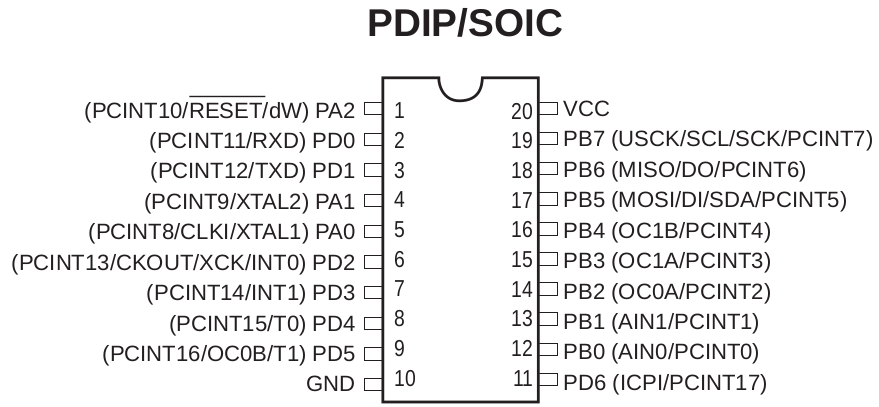
\includegraphics[width=0.5\textwidth]{images/pines.png}
    \caption{Diagrama de pines del ATtiny4313 \cite{datasheet}}
    \label{pines}
\end{figure}

\begin{figure}[H]
    \centering
    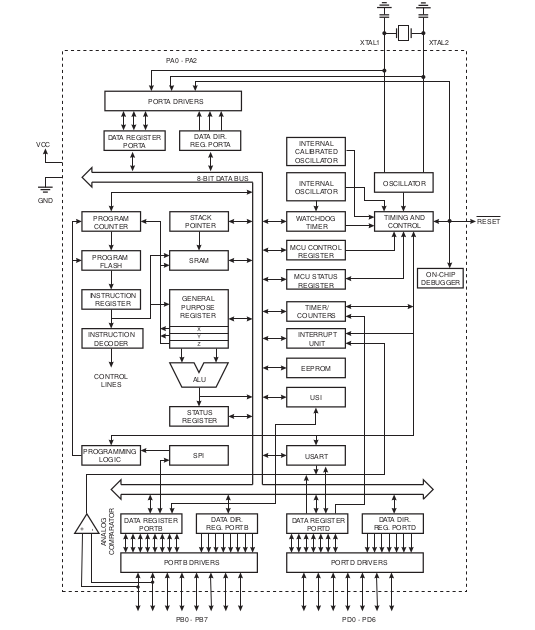
\includegraphics[width=0.5\textwidth]{images/bloques.png}
    \caption{Diagrama de bloques del ATtiny4313 \cite{datasheet}}
    \label{bloques}
\end{figure}